\documentclass[../TDE4-E5.tex]{subfiles}%

\begin{document}
\section[s]"3"{Décrément logarithmique mécanique}

\enonce{%
	\noindent
	\begin{minipage}{0.49\linewidth}
		Une masse $m$ est accrochée à un ressort de raideur $k = \SI{10}{N.m^{-1}}$
		et de longueur à vide $\ell_0 = \SI{10}{cm}$, fixé au point $O$. En plus de
		son poids et de la force de rappel du ressort, la masse est soumise à une
		force de frottement fluide $\Ff = -\alpha\vv{v}$. Un capteur fournit
		l'évolution de $u(t) = z(t)-z_{\rm eq}$ au court du temps.
	\end{minipage}
	\begin{minipage}{0.49\linewidth} \centering
		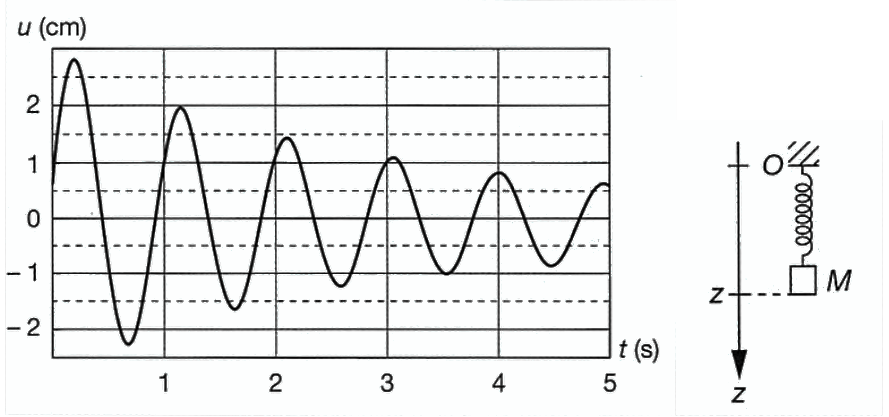
\includegraphics[width=\linewidth]{dec_log-courbe_meca}
	\end{minipage}
}%

\QR{%
	Établir l'équation d'évolution de $z(t)$. Quelle est la position d'équilibre
	$z_{\rm eq}$ de la masse ? En déduire une équation satisfaite par $u(t)$.
}{%
	On repère par $z(t)$ l'altitude du ressort. Étant donné le système, le
	mouvement ne s'effectue que selon $\uz$, et on a $v = \dv{z}{t}$ et $a =
		\dv[2]{z}{t}$. De plus, la longueur $\ell$ du ressort s'identifie à
	l'altitude $z(t)$ de la masse. On effectue donc le \textbf{bilan des forces}
	en faisant attention au sens de $\uz$~:
	\[
		\begin{array}{ll}
			\textbf{Poids}      & \Pf = mg\uz                                \\
			\textbf{Ressort}    & \vv*{F}{\rm ressort} = -k (z(t)-\ell_0)\uz \\
			\textbf{Frottement} & \Ff = -\alpha \dv{z}{t}\uz
		\end{array}
	\]
	Ainsi, le \textbf{PFD} donne
	\begin{gather*}
		m \dv[2]{z}{t} = mg - k(z(t)-\ell_0) -\alpha \dv{z}{t}
		\Lra
		\boxed{m\dv[2]{z}{t} + \alpha \dv{z}{t} + kz = mg + k\ell_0}
	\end{gather*}
	À l'équilibre, $\dv{z}{t} = 0$ et $\dv[2]{z}{t} = 0$, on trouve donc
	\begin{equation*}
		z_{\rm eq} = \ell_0 + \frac{mg}{k}
	\end{equation*}
	À cause du poids qui n'est cette fois pas compensé par la réaction du support,
	la longueur d'équilibre est plus grande que la longueur à vide du ressort. On
	réexprime l'équation différentielle avec le changement de variable de l'énoncé
	pour avoir
	\begin{gather*}
		\boxed{m\dv[2]{u}{t} + \alpha \dv{u}{t} + ku = 0}
	\end{gather*}
}%

\QR{%
	Exprimer la pulsation propre $\w_0$ et le facteur de qualité $Q$ en
	fonction des données du problème.
}{%
	On met l'équation sous forme canonique et on identifie~:
	\begin{equation*}
		\boxed{ \dv[2]{u}{t} + \frac{\w_0}{Q} \dv{u}{t} + \w_0{}^2u = 0}
		\qavec
		\boxed{\w_0 = \sqrt{\frac{k}{m}}}
		\qet
		\boxed{Q = \frac{\sqrt{km}}{\alpha}}
	\end{equation*}
}%

\QR{%
	Résoudre l'équation différentielle. Exprimer la pseudo-période $T$ en
	fonction de $T_0 = \DS \frac{2\pi}{\w_0}$ et de $Q$.
}{%
	On exprime l'équation caractéristique de discriminant $\Delta$~:
	\begin{gather*}
		r^2 + \frac{\w_0}{Q}r + \w_0{}^2 = 0 \Rightarrow \Delta = \w_0{}^2
		\left( \frac{1}{Q^2} - 4 \right)
	\end{gather*}
	On observe des oscillations, donc $\Delta < 0$. Les racines sont donc
	\begin{gather*}
		\boxed{r_\pm = -\frac{\w_0}{2Q} \pm \jj \w}
		\qavec
		\boxed{\w = \w_0 \sqrt{1 - \frac{1}{Q^2}}}
	\end{gather*}
	et les solutions sont de la forme
	\begin{equation*}
		\boxed{z(t) = \exr^{- \frac{\w_0}{2Q}t} \left[ A\cos\wt + B\sin\wt \right]}
	\end{equation*}
	Sans conditions initiales, on ne peut déterminer $A$ et $B$. On peut
	cependant exprimer $T$~:
	\begin{equation*}
		\boxed{T = \frac{2\pi}{\w} = \frac{T_0}{\sqrt{1 - \frac{1}{4Q^2}}}}
	\end{equation*}
}

\QR{%
Montrer que le décrément logarithmique $\delta$, défini par
\[\boxed{ \delta = \frac{1}{n} \ln \left( \frac{u(t) -
	u_{\rm eq}}{u(t+nT)-u_{\rm eq}} \right)}\]
est indépendant du temps.
}{%
Par construction, $u_{\rm eq} = 0$, et on a
\begin{gather*}
	u(t+nT) = \exr^{- n\frac{\w_0}{2Q}T}\times
	\underbracket[1pt]{\exr^{- \frac{\w_0}{2Q}t}
		\left[ A\underset{=\cos\wt}{\underline{\cos(\w(t+nT))}} +
			B\underset{=\sin\wt}{\underline{\sin(\w(t+nT))}} \right]
	}_{=u(t)}
	\Leftrightarrow u(t+nT) = \exr^{-n \frac{\w_0}{2Q}T}u(t)
\end{gather*}
Ainsi,
\begin{gather*}
	\delta = \frac{1}{n}\ln \left( \frac{u(t)}{\exr^{-n\frac{\w_0}{2Q}T}u(t)}
	\right) = \frac{1}{n}\ln \left( \exr^{n \frac{\w_0}{2Q}T} \right)\\
	\Leftrightarrow \boxed{\delta = \frac{\w_0}{2Q}T}
\end{gather*}
En développant $T$ on trouve
\begin{gather*}
	\delta = \frac{1}{2Q} \frac{\overbracket[1pt]{\w_0T_0}^{=2\pi}}{\sqrt{1 -
			\frac{1}{4Q^2}}}
	\Leftrightarrow
	\boxed{\delta = \frac{2\pi}{\sqrt{4Q^2-1}}}
\end{gather*}
ce qui est bien indépendant du temps $t$.
}%

\QR{%
	Comparer les données expérimentales à l'affirmation précédente. Commenter.
}{%
	Soit $t_{\max}$ le temps du premier maximum. On relève les ordonnées des
	maximums successifs de $u(t)$, c'est-à-dire $u(t_{\max} + nT)$, et on calcule
	le logarithme népérien de deux longueurs successives~:
	\begin{center}
		\begin{tabular}{lcc}
			\toprule
			$n$ & $u(t_{\max} + nT)$ & $\delta$   \\
			\midrule
			0   & \num{2.9}          & \num{0.37} \\
			1   & \num{2.0}          & \num{0.29} \\
			2   & \num{1.5}          & \num{0.31} \\
			3   & \num{1.1}          & \num{0.31} \\
			4   & \num{0.8}          & \num{0.29} \\
			5   & \num{0.6}          &            \\
			\bottomrule
		\end{tabular}
	\end{center}
	Mise à part la première valeur, les résultats sont assez peu dispersés. Cela
	valide bien le modèle d'oscillateur amorti pour cette expérience~; l'écart
	de la première valeur est sûrement lié à des non-linéarités du ressort aux
	longueurs importantes.
}%

\QR{%
	Estimer à l'aide des données expérimentales le facteur de qualité $Q$ et
	la pseudo-pulsation $\w$.
}{%
	On peut donc estimer qu'on a $\delta = \num{0.30\pm0.01}$. On isole $Q$ de son
	expression~:
	\begin{gather*}
		\delta = \frac{2\pi}{\sqrt{4Q^2-1}}
		\Leftrightarrow
		\sqrt{4Q^2 - 1}^2 = \left( \frac{2\pi}{\delta} \right)^2
		\Leftrightarrow
		4Q^2 = 1+ \left( \frac{2\pi}{\delta} \right)^2\\
		\Leftrightarrow
		\boxed{Q = \sqrt{ \frac{\pi^2}{\delta^2}+ \frac{1}{4}}}\\
		\text{A.N.~:~} \boxed{Q \approx \num{10.5}}
	\end{gather*}
	On trouve bien $Q \gg 0.5$ comme le montre l'oscillogramme. Quant à $\w$, on
	peut estimer $T$ en comptant plusieurs périodes~: on a $t_{\max} =
		\SI{0.2}{s}$ et $t_{\max} + 5T = \SI{4.9}{s}$, donc on a $5T = \SI{4.2}{s}$,
	c'est-à-dire \fbox{$T \approx \SI{0.95}{s}$}. Enfin, $\w = 2\pi/T$, donc
	\begin{equation*}
		\boxed{\w = \SI{6.6}{rad.s^{-1}}}
	\end{equation*}
}%

\QR{%
	En déduire les valeurs de $m$ et $\alpha$.
}{%
	Comme $Q \gg 0.5$, on a $\w \approx \w_0 = \sqrt{\frac{k}{m}}$. On a donc
	\begin{gather*}
		\boxed{m \approx \frac{k}{\w^2}}
		\qavec
		\left\{
		\begin{array}{rcl}
			k  & = & \SI{10}{N.m^{-1}}    \\
			\w & = & \SI{6.6}{rad.s^{-1}}
		\end{array}
		\right.\\
		\text{A.N.~:~} \boxed{m \approx \SI{230}{g}}
	\end{gather*}
	Finalement, on a
	\begin{gather*}
		\boxed{\alpha = \frac{\sqrt{km}}{Q}}
		\qavec
		\left\{
		\begin{array}{rcl}
			k & = & \SI{10}{N.m^{-1}} \\
			m & = & \SI{230}{g}       \\
			Q & = & \num{10.5}
		\end{array}
		\right.\\
		\text{A.N.~:~} \boxed{\alpha \approx \SI{0.15}{kg.s^{-1}}}
	\end{gather*}
}%

\end{document}
